\subsection{Value Function and the Definition of Rewards}
Having updated the belief state, the system must again pick the next action.
Remember that our system aims to maximize the single-number metric of the area under the AP vs. Time curve.
Accordingly, we define the final reward accrued by a policy to be precisely the area under the curve between start and deadline times.

\begin{figure}[htb]
  \center{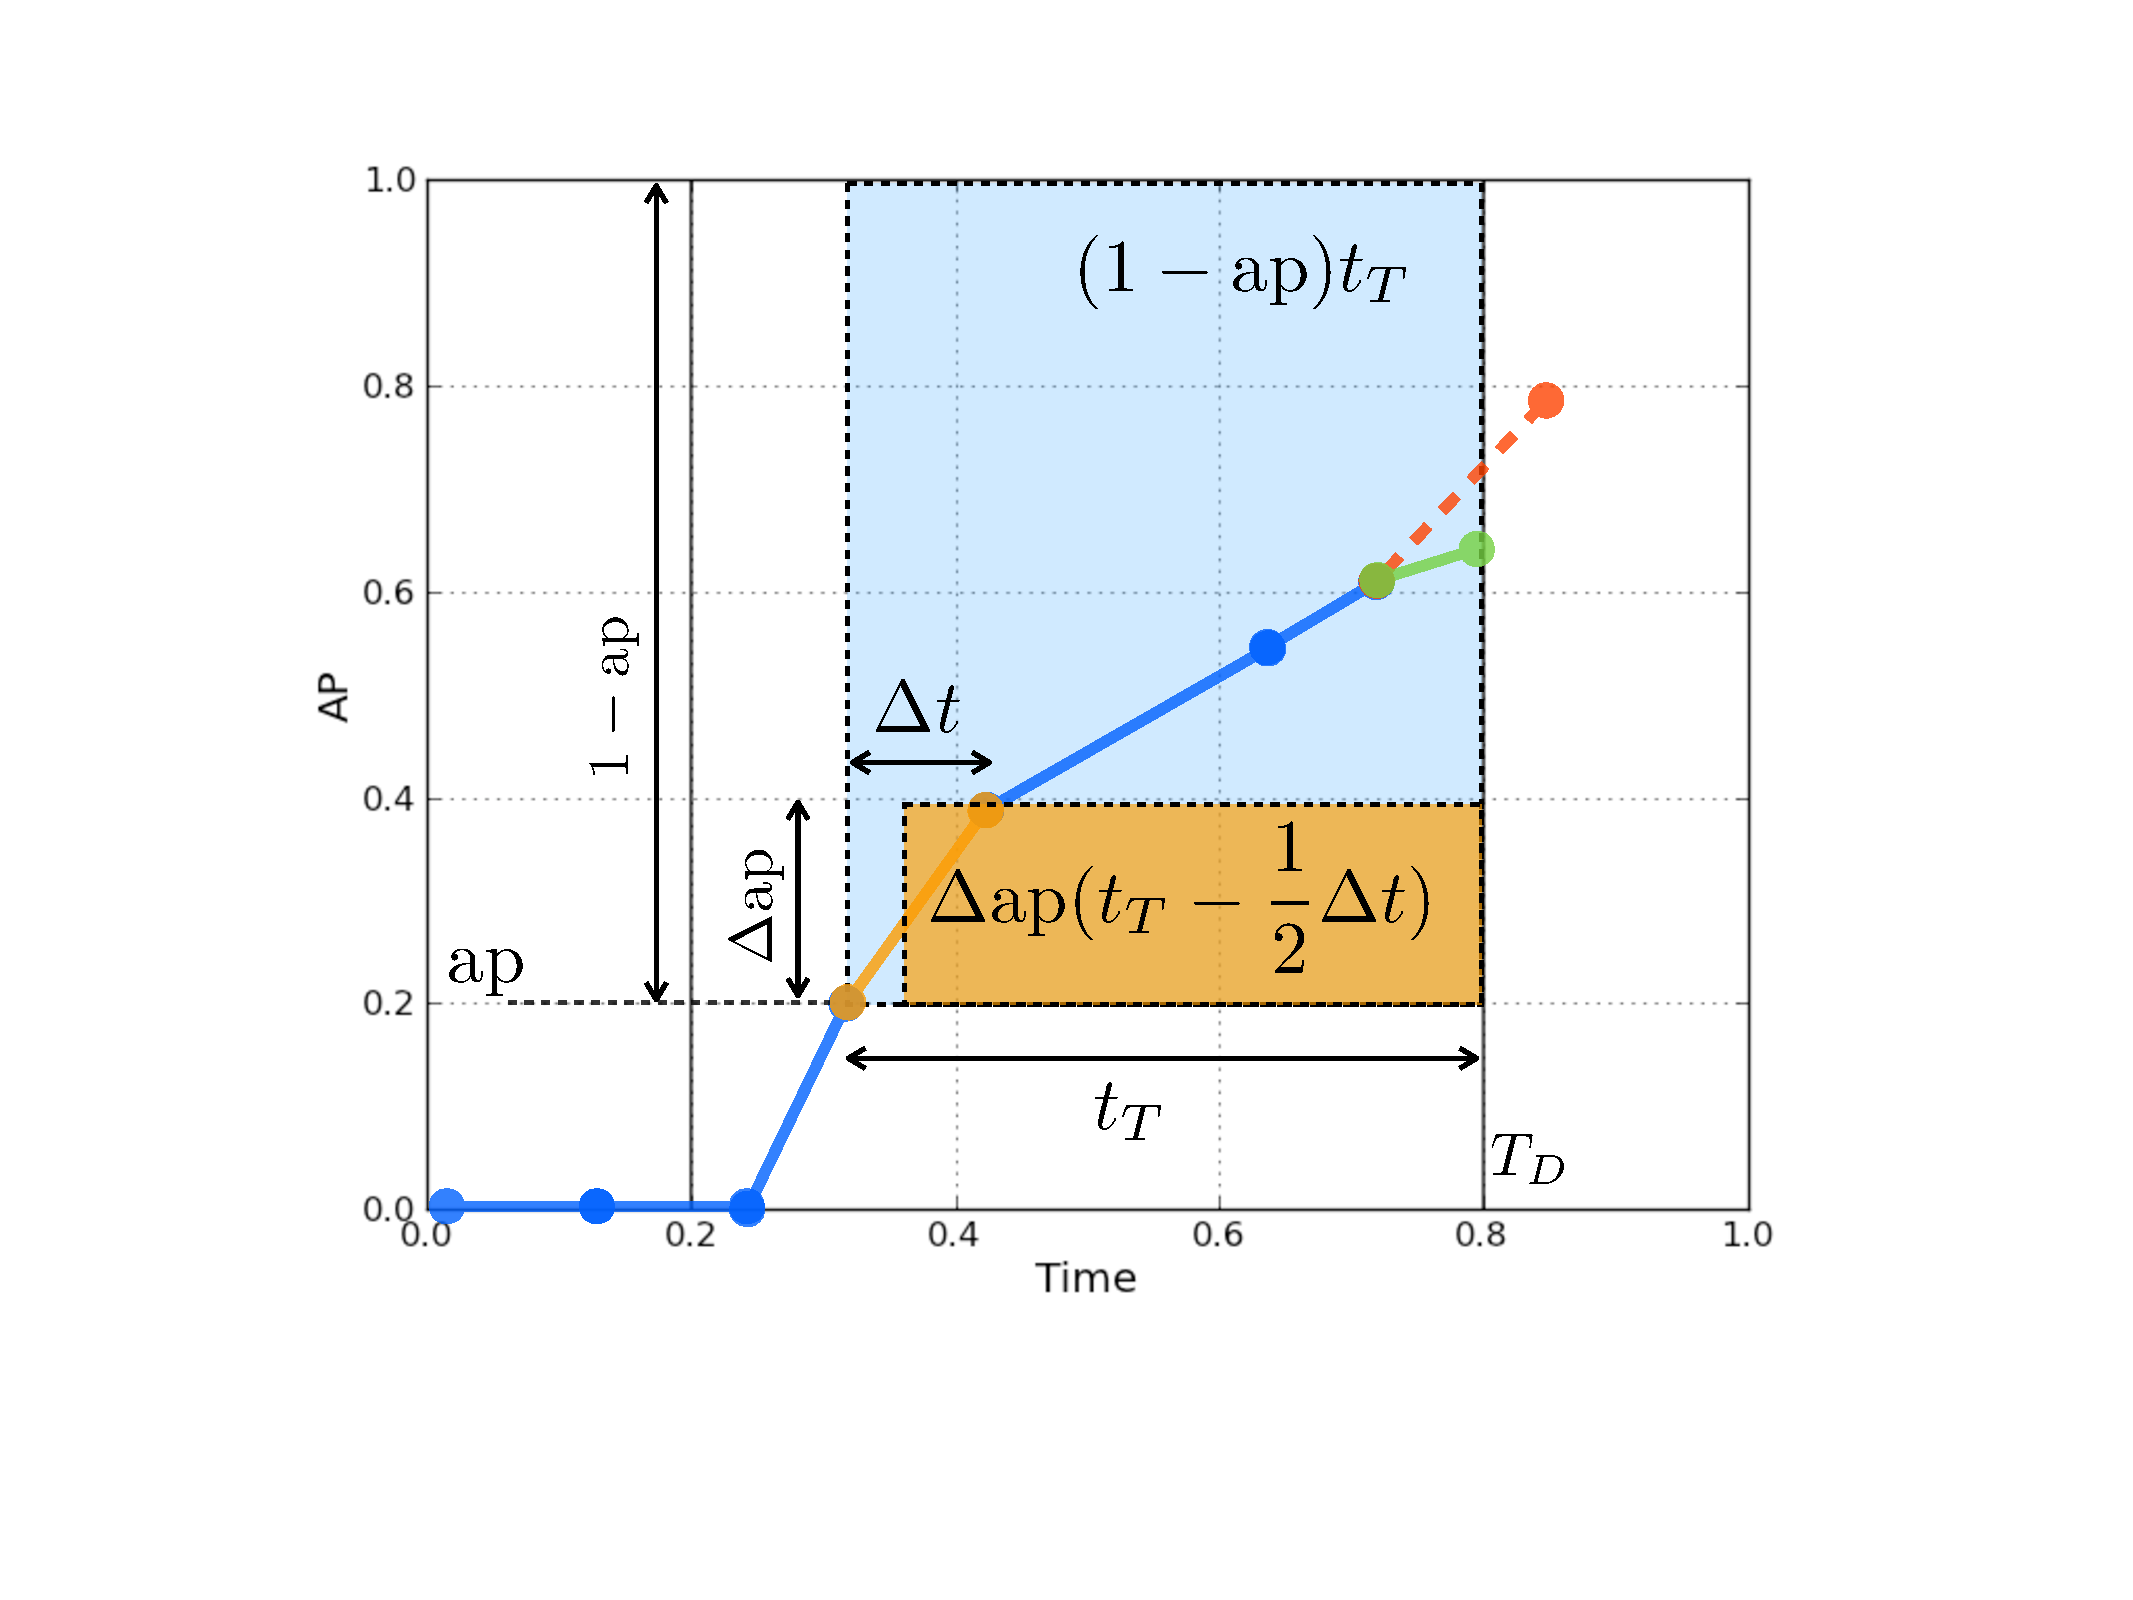
\includegraphics[width=1\linewidth]{figures/apvst_expl.pdf}}
  \caption{\label{fig:rewards}A per-action greedy value function that corresponds to the maximization of our objective function is the ratio of the area of the horizontal slice under the curve due to the action to the maximum possible area the action could have captured. The figure shows this analysis for the action highlighted in orange.}
\end{figure}

The final reward of the policy should be the summation of individual rewards accrued by each action.
Our choice, shown in Figure~\ref{fig:rewards}, is the area of a horizontal ``slice'' of the area under the curve due to the action.

Specifically, we define the reward of an action as
\begin{equation}\label{eq:advanced}
\Delta AP (t_T-\Delta t)
\end{equation}
where $t_T$ is the time left until deadline, and $\Delta t$ and $\Delta AP$ are the time taken and AP change produced by the action.

The equation breaks down into a term to maximize, $\Delta AP t_T$, and a term to minimize, $\Delta AP \Delta t$.
This agrees with the intuition that to capture the most area under the curve, the slope needs to be maximized at each point.
Additionally, the equation shows that if $\Delta t$ exceeds $t_T$, the value of taking the action is negative.
This is good, as these actions don't actually contribute detections to the final evaluation.

We can accentuate the desire for high slope in a value function with the same properties:
\begin{equation}\label{eq:slope}
\frac{\Delta AP}{\Delta t} (t_T - \Delta t)
\end{equation}
This function always maximizes the slope, except for when doing so would lead to taking more time than alloted by the deadline.
(Consider the branching of the performance curve in \ref{fig:rewards} into green and red branches when it approaches the deadline.
The branches represent two actions of the case where maximizing slope would not be the correct behavior.)

Of course, we cannot be aware of the true value of $\Delta t$ until having taken the action, and the policy can never be fully certain of the value of $\Delta AP$.
When estimating the value function, we therefore use the expected values of these terms.

$\Delta t_{avg}$ is the average running time of the detector on an image, estimated on a validation set of the data at training time.
$\Delta AP$ is estimated as $\Delta AP_{avg} P(C)$, where $P(C)$ is the current belief in the presence of class $C$ in the image, and $\Delta AP_{avg}$ is the ``naive'' AP contribution averaged over images containing class $C$.

During training time, we learn the behavior of different detectors: the average time taken per image, and the average AP contribution on images that do and do not contain any objects of the desired class.
For the latter statistic, we collect two variants.
The ``naive'' AP contribution is the performance of the detector in the multi-class regime if its detections were added to an empty set of detections.
That is, true detections cannot become false positives due to being overshadows by a more confident but wrong detection of a different class in this evaluation.

The ``actual'' AP contribution is the real performance of the detector in the multi-class regime: its detections are added to an existing set of detections, unless it was the result of the first action to run.
This case, although more realistic, is subject to signficant noise due to other detectors' performance that may obscure the evaluated detector's characteristics.


We additionally experimented with estimating $\Delta AP$ as $\Delta AP_{avg|present} P(C) + \Delta AP_{avg|absent} (1-P(C))$, but the results were worse than with the given equation.
